% !TeX spellcheck = ru_RU
\documentclass[a4paper,12pt]{extarticle}
\usepackage[utf8x]{inputenc}
\usepackage[T1,T2A]{fontenc}
\usepackage[russian]{babel}
\usepackage{hyperref}
\usepackage{indentfirst}
\usepackage{listings}
\usepackage{color}
\usepackage{here}
\usepackage{array}
\usepackage{multirow}
\usepackage{graphicx}

\usepackage{caption}
\renewcommand{\lstlistingname}{Программа} % заголовок листингов кода

\bibliographystyle{ugost2008ls}

\usepackage{listings}
\lstset{ %
extendedchars=\true,
keepspaces=true,
language=C,						% choose the language of the code
basicstyle=\footnotesize,		% the size of the fonts that are used for the code
numbers=left,					% where to put the line-numbers
numberstyle=\footnotesize,		% the size of the fonts that are used for the line-numbers
stepnumber=1,					% the step between two line-numbers. If it is 1 each line will be numbered
numbersep=5pt,					% how far the line-numbers are from the code
backgroundcolor=\color{white},	% choose the background color. You must add \usepackage{color}
showspaces=false				% show spaces adding particular underscores
showstringspaces=false,			% underline spaces within strings
showtabs=false,					% show tabs within strings adding particular underscores
frame=single,           		% adds a frame around the code
tabsize=2,						% sets default tabsize to 2 spaces
captionpos=t,					% sets the caption-position to top
breaklines=true,				% sets automatic line breaking
breakatwhitespace=false,		% sets if automatic breaks should only happen at whitespace
escapeinside={\%*}{*)},			% if you want to add a comment within your code
postbreak=\raisebox{0ex}[0ex][0ex]{\ensuremath{\color{red}\hookrightarrow\space}},
texcl=true,
inputpath=listings,                     % директория с листингами
}

\usepackage[left=2cm,right=2cm,
top=2cm,bottom=2cm,bindingoffset=0cm]{geometry}

%% Нумерация картинок по секциям
\usepackage{chngcntr}
\counterwithin{figure}{section}
\counterwithin{table}{section}

%%Точки нумерации заголовков
\usepackage{titlesec}
\titlelabel{\thetitle.\quad}
\usepackage[dotinlabels]{titletoc}

%% Оформления подписи рисунка
\addto\captionsrussian{\renewcommand{\figurename}{Рисунок}}
\captionsetup[figure]{labelsep = period}

%% Подпись таблицы
\DeclareCaptionFormat{hfillstart}{\hfill#1#2#3\par}
\captionsetup[table]{format=hfillstart,labelsep=newline,justification=centering,skip=-10pt,textfont=bf}

%% Путь к каталогу с рисунками
\graphicspath{{fig/}}
\usepackage{minted}

\begin{document}	% начало документа
	
	% Титульная страница
	\begin{titlepage}	% начало титульной страницы

	\begin{center}		% выравнивание по центру

		\large Санкт-Петербургский политехнический университет Петра Великого\\
		\large Институт компьютерных наук и технологий \\
		\large Кафедра компьютерных систем и программных технологий\\[6cm]
		% название института, затем отступ 6см
		
		\huge Телекоммуникационные технологии\\[0.5cm] % название работы, затем отступ 0,5см
		\large Отчет по лабораторной работе №6\\[0.1cm]
		\large Цифровая модуляция\\[5cm]

	\end{center}


	\begin{flushright} % выравнивание по правому краю
		\begin{minipage}{0.25\textwidth} % врезка в половину ширины текста
			\begin{flushleft} % выровнять её содержимое по левому краю

				\large\textbf{Работу выполнил:}\\
				\large Косенков М.А.\\
				\large {Группа:} 33531/2\\
				
				\large \textbf{Преподаватель:}\\
				\large Богач Н.В.

			\end{flushleft}
		\end{minipage}
	\end{flushright}
	
	\vfill % заполнить всё доступное ниже пространство

	\begin{center}
	\large Санкт-Петербург\\
	\large \the\year % вывести дату
	\end{center} % закончить выравнивание по центру

\thispagestyle{empty} % не нумеровать страницу
\end{titlepage} % конец титульной страницы

\vfill % заполнить всё доступное ниже пространство
	
	% Содержание
	\setcounter{page}{2}
	% Содержание
\renewcommand\contentsname{\centerline{Содержание}}
\tableofcontents
\newpage
	
	
	\section{Цель работы}
	Изучение методов модуляции цифровых сигналов.
	
	\section{Программа работы}
	\begin{itemize}
		\item Получить сигналы BPSK, QPSK, 8-PSK, DBPSK, DQPSK и QAM модуляторов
		\item Построить их сигнальные созвездия
		\item Провести сравнение изученных методов модуляции цифровых сигналов.
	\end{itemize}
	
	\section{Теоретическая информация}
	Модуляция (лат. modulatio — размеренность, ритмичность) — процесс изменения одного или нескольких параметров модулируемого несущего сигнала при помощи модулирующего сигнала.
	
	В цифровой модуляции аналоговый несущий сигнал модулируется цифровым битовым потоком.
	Существуют три фундаментальных типа цифровой модуляции (или шифтинга) и один гибридный:
	\begin{itemize}
		\item ASK – Amplitude shift keying (Амплитудная двоичная модуляция).
		\item FSK – Frequency shift keying (Частотая двоичная модуляция).
		\item PSK – Phase shift keying (Фазовая двоичная модуляция).
		\item ASK/PSK.
	\end{itemize}
	
	Стоит упомянуть, что в русской терминологии радиосвязи существует традиция использовать для модуляции цифровым сигналом термин «манипуляция».
	
	\begin{figure}[H]
		\begin{center}
			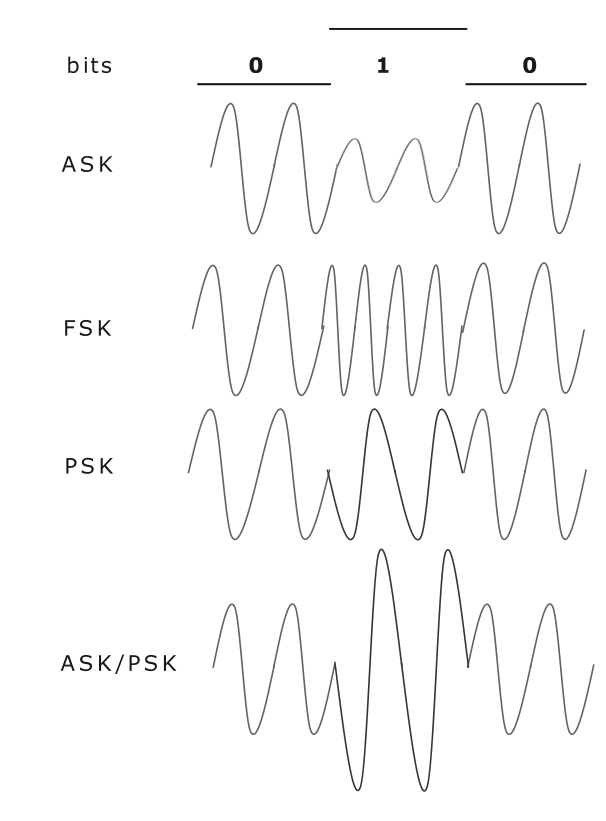
\includegraphics[width=0.4\linewidth]{../modulations}
			\caption{Виды манипуляций}
		\end{center}
	\end{figure}
	
	В случае амплитудного шифтинга амплитуда сигнала для логического нуля может быть (например) в два раза меньше логической единицы.
	
	Частотная модуляция похожим образом представляет логическую единицу интервалом с большей частотой, чем ноль.
	
	Фазовый шифтинг представляет «0» как сигнал без сдвига, а «1» как сигнал со сдвигом.
	
	Каждая из схем имеет свои сильные и слабые стороны.
	\begin{itemize}
		\item ASK хороша с точки зрения эффективности использования полосы частот, но подвержена искажениям при наличии шума и недостаточно эффективна с точки зрения потребляемой мощности.
		\item FSK – с точностью до наоборот, энергетически эффективна, но не эффективно использует полосу частот.
		\item PSK – хороша в обоих аспектах.
		\item ASK/PSK – комбинация двух схем. Она позволяет еще лучше использовать полосу частот.
	\end{itemize}
	
	Самая простая PSK схема (показанная на рисунке) имеет собственное название — Binary phase-shift keying. Используется единственный сдвиг фазы между «0» и «1» — 180 градусов, половина периода.
	
	Существуют также QPSK и 8-PSK:
	
	QPSK использует 4 различных сдвига фазы (по четверти периода) и может кодировать 2 бита в символе (01, 11, 00, 10). 8-PSK использует 8 разных сдвигов фаз и может кодировать 3 бита в символе. 
	
	Одна из частных реализаций схемы ASK/PSK которая называется QAM — Quadrature Amplitude Modulation (квадратурная амплитудная модуляция (КАМ). Это метод объединения двух AM-сигналов в одном канале. Он позваляет удвоить эффективную пропускную способность. В QAM используется две несущих с одинаковой частотой но с разницей в фазе на четверть периода (отсюда и возникает слово квадратура). Более высокие уровни QAM строятся по тому же принципы, что и PSK.
	
	Кроме того, существуют также дифференциальные фазовые манипуляции. Их отличие от PSK состоит в том, что декодирование сигнала происходит не по абсолютному значению фазы, а по относительному. Таким образом, каждый последующий бит кодируется изменением фазы относительно предыдущего. Это позволяет избежать таких сильных фазовых скачков, как в BPSK.

	\newpage
	\section{Ход работы}
	Данная работа выполнялась с использованием графической среды GNURadio.
	\par
	Были рассмотрены различные виды манипуляций, а именно - фазовые манипуляции BPSK, QPSK, 8PSK, а также квадратурная манипуляция 16QAM и дифференциальные фазовые манипуляции DBPSK и DQPSK. Ниже приведены схемы в среде GNURadio, позволяющие сгенерировать требуемые сигналы.
	\par
	\begin{center}
		\large {Фазовые манипуляции}
	\end{center}
		\begin{figure}[H]
		\begin{center}
			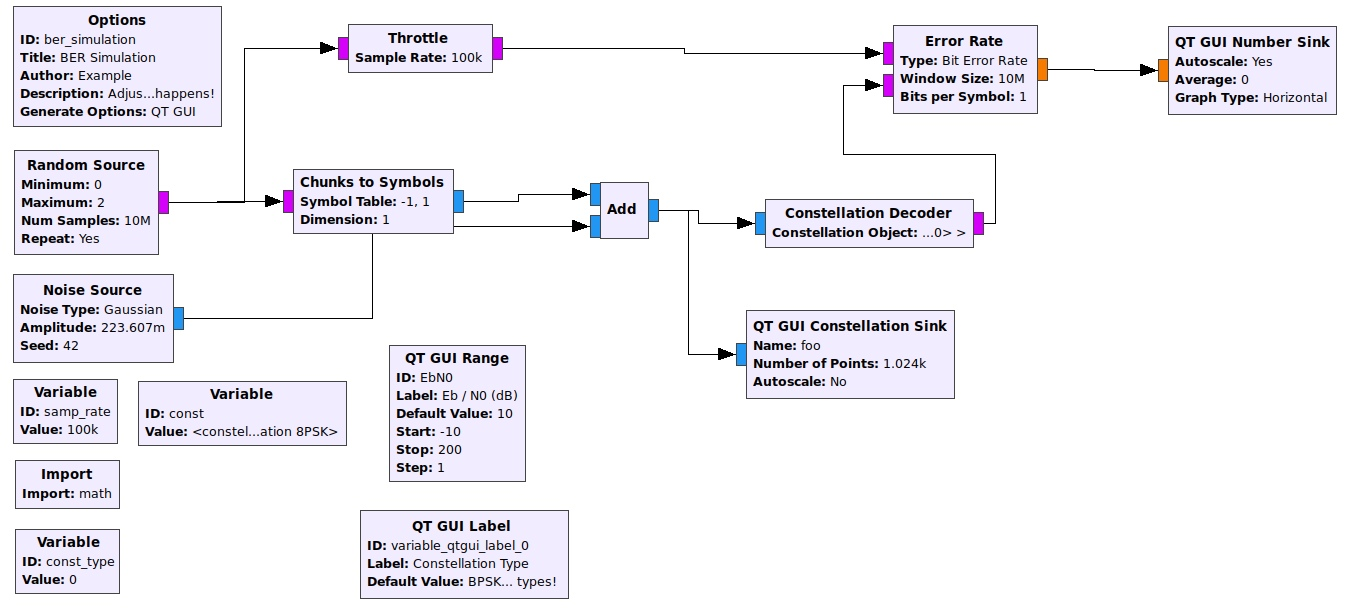
\includegraphics[scale=0.35]{../pks_graph.jpg}
			\caption{Схема модуляции M-PSK, M-количество дискретных значений} 
		\end{center}
	\end{figure}

	\begin{center}
	\large {Дифференциальные фазовые манипуляции}
	\end{center}
	\begin{figure}[H]
		\begin{center}
			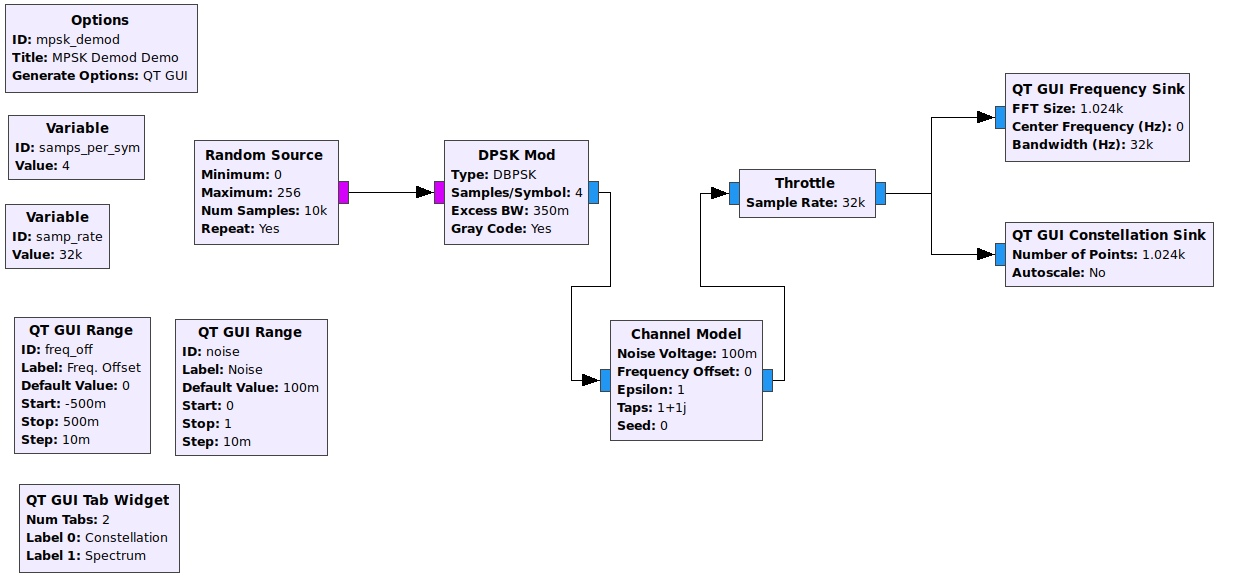
\includegraphics[scale=0.4]{../dpsk_graph.jpg}
			\caption{Схема модуляции DBPSK и DQPSK} 
		\end{center}
	\end{figure}

	\large {Результат работы}
	\begin{center}
		\large {Фазовые манипуляции}
	\end{center}
	Для демонстрации особенностей PSK-манипуляций, сначала посмотрим, как будет выглядеть сигнальное созвездие BPSK с маленьким шумом и с сильным.
	
	\begin{figure}[H]
		\begin{center}
			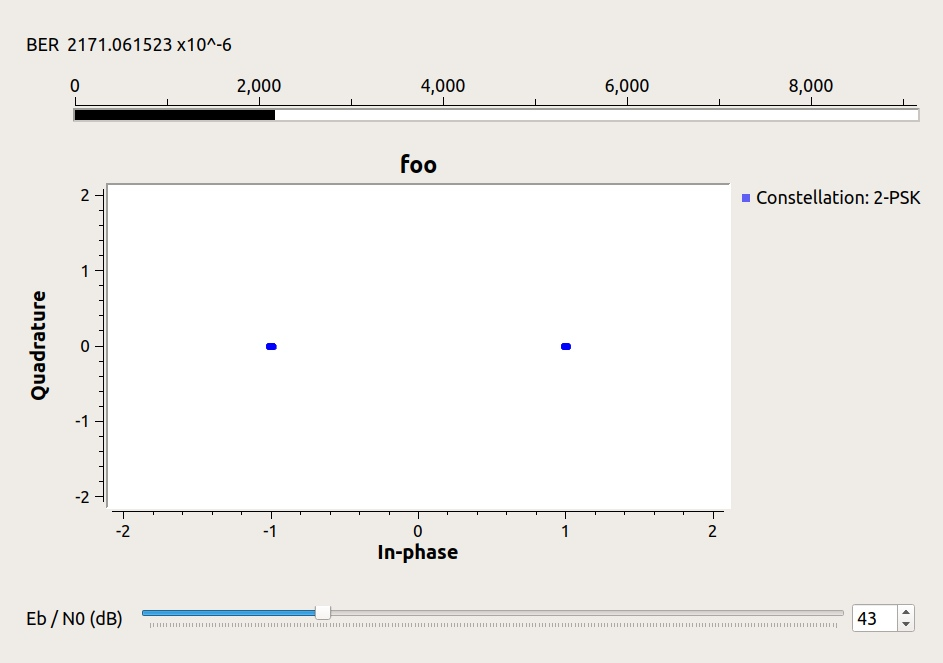
\includegraphics[scale=0.4]{../bpsk.jpg}
			\caption{Сигнальное созвездие BPSK} 
		\end{center}
	\end{figure}
	
	\begin{figure}[H]
		\begin{center}
			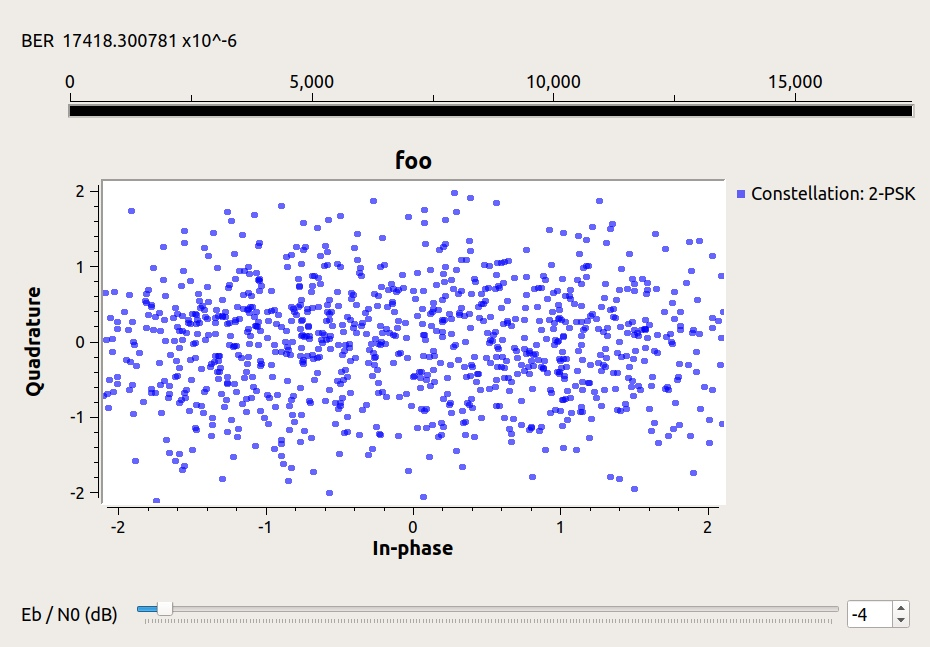
\includegraphics[scale=0.4]{../bpsk_noisy.jpg}
			\caption{BPSK в сильно зашумленном канале} 
		\end{center}
	\end{figure}
	
	Как можно видеть, при высоком отношении сигнал/шум облака разброса минимальны, что позволяет в абсолютном большинстве случаев декодировать передаваемый бит. Однако при отрицательном отношении сигнал/шум эти облака перекрывают друг друга и количество ошибок начинает стремительно расти, заполняя собой всю шкалу. 

	\begin{figure}[H]
		\begin{center}
			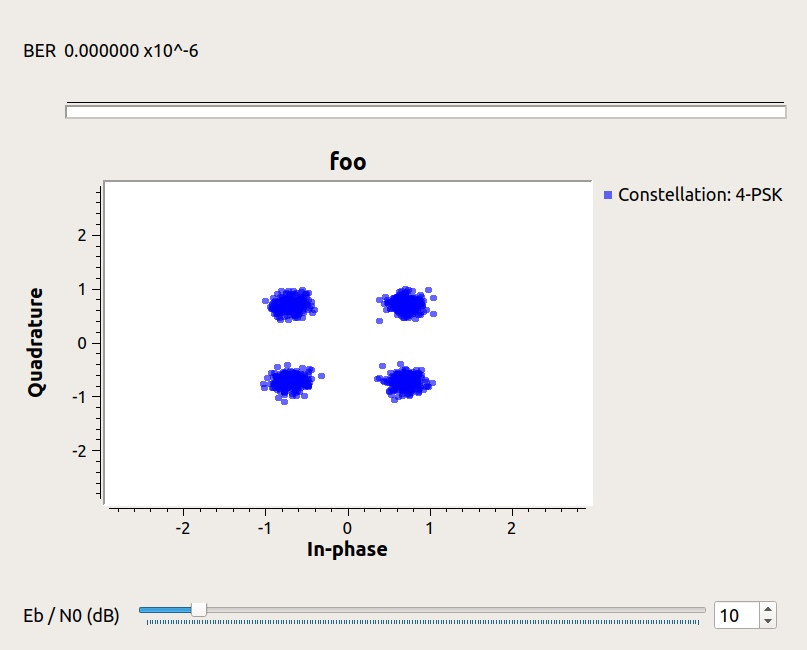
\includegraphics[scale=0.4]{../qpks.jpg}
			\caption{Сигнальное созвездие QPSK} 
		\end{center}
	\end{figure}

	Теперь сравним BPSK с QPSK. Мы выигрываем в количестве передаваемой информации, однако требуемое отношение сигнал/шум стало чуть больше. Тем не менее, при 10 Db мы все еще можем наблюдать четкие 4 точки. Если уменьшить отношение, облака опять станут сливаться в одну большую область.

	\begin{figure}[H]
		\begin{center}
			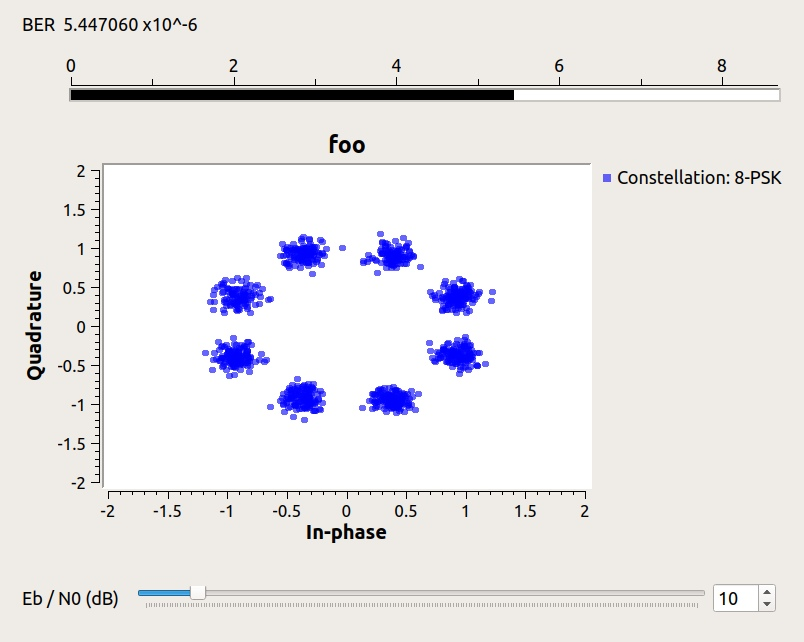
\includegraphics[scale=0.4]{../8psk.jpg}
			\caption{Сигнальное созвездие 8-PSK} 
		\end{center}
	\end{figure}

	При манипуляции 8-PSK мы еще больше выигрываем в количестве передаваемой информации, однако теперь при тех же 10 Db, которых было достаточно для QPSK, мы наблюдаем рост числа ошибок. Это означает, что нужно либо уменьшить количество дискретных значений, либо увеличить отношение сигнал/шум.
	
	\begin{center}
		\large {Дифференциальная фазовая манипуляция}
	\end{center}
	
	\begin{figure}[H]
		\begin{center}
			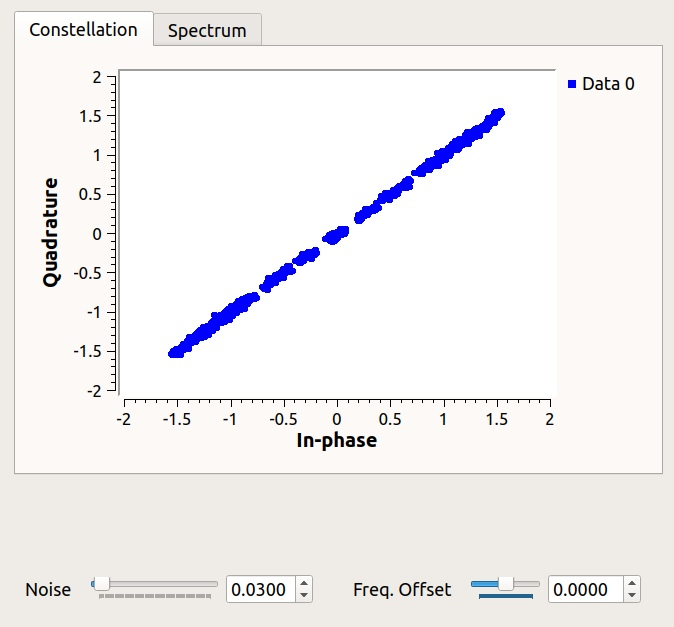
\includegraphics[scale=0.4]{../dbpsk.jpg}
			\caption{Сигнальное созвездие DBPSK} 
		\end{center}
	\end{figure}
	Сигнальное созвездие отличается от BPSK, поскольку на нем отражены также промежуточные точки - переходные. Это приводит к тому, что мы видим почти линию, т.к. значений у нас всего 2 и все промежуточные точки лежат между ними. Это является отличительной особенностью дифференциальной фазовой манипуляции, т.к., как было сказано ранее, каждый последующий бит зависит от фазы предыдущего. Кроме того, мы видим, что наклон прямой не такой, как был в BPSK. Это происходит из-за фазового сдвига.

	\begin{figure}[H]
		\begin{center}
			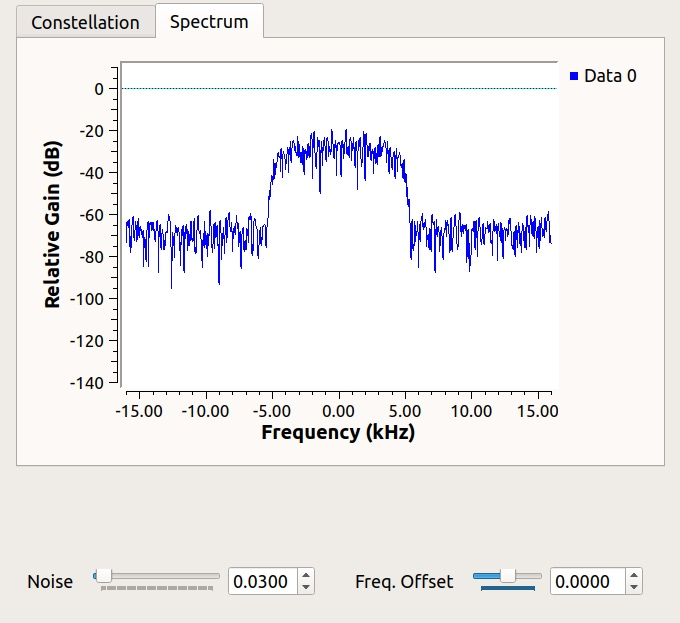
\includegraphics[scale=0.4]{../dbpsk_spectrum.jpg}
			\caption{Спектр DBPSK} 
		\end{center}
	\end{figure}
	Здесь мы можем управлять фазовым сдвигом, контролируя спектр модулируемого сигнала и, соответственно, наклон сигнального созвездия. Поменять сдвиг попробуем в DQPSK, созвездие которого является, на мой взгляд, самым красивым среди всех сравниваемых.

	\begin{figure}[H]
		\begin{center}
			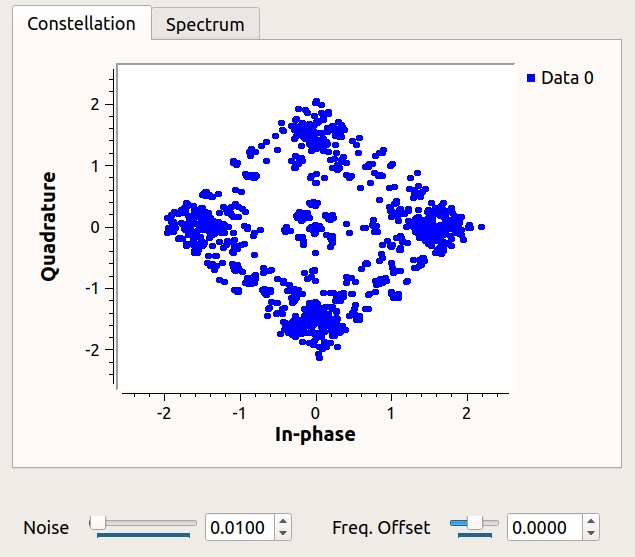
\includegraphics[scale=0.4]{../dqpsk.jpg}
			\caption{Сигнальное созвездие DQPSK} 
		\end{center}
	\end{figure}
	Как можно заметить, созвездие опять отличается не только наличием промежуточных точек, но и расположением эталонных дискретных значений. По сути, в QPSK имеются те же самые значения, но они из-за другой фазы, они представляют из себя квадрат. Здесь же получился ромб, что, как мне кажется, даже более приятно глазу. 
	\par
	Однако, помимо созерцания, мы попробуем сдвинуть фазу. По расчетам, мы увидим не только сдвиг на спектральном графике, но и изменившийся угол наклона квадрата в созвездии.
	\begin{figure}[H]
		\begin{center}
			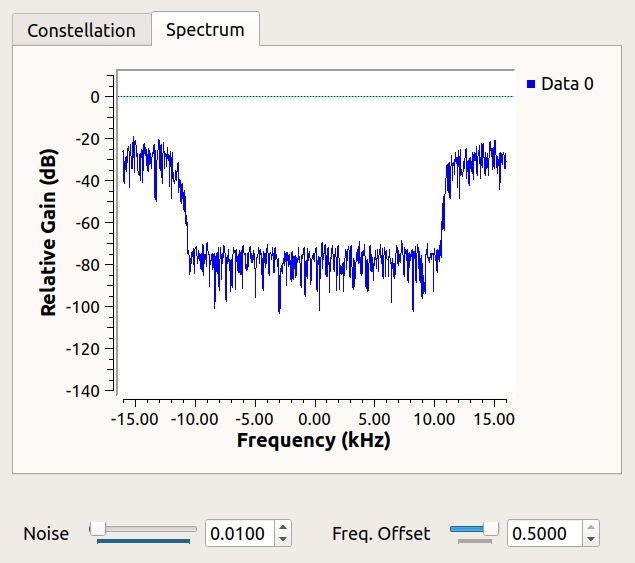
\includegraphics[scale=0.4]{../dqpsk_spectrum.jpg}
			\caption{Спектр DQPSK со сдвигом 0.5} 
		\end{center}
	\end{figure}
		\begin{figure}[H]
		\begin{center}
			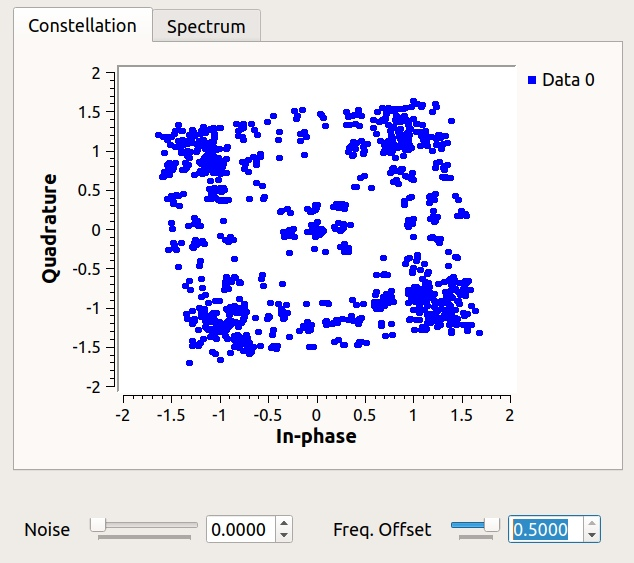
\includegraphics[scale=0.4]{../dqpsk_shift.jpg}
			\caption{Сигнальное созвездие DQPSK со сдвигом 0.5} 
		\end{center}
	\end{figure}
	Очевидно, что у нас получилось сделать то, что мы хотели. Сдвиг фазы повлек за собой изменение сигнального созвездия. Таким образом, мы можем настраивать нужные нам значения, основываясь на информации о характеристиках канала, чтобы сделать передачу максимально эффективной.
	\par
	Тем не менее, сдвиг фазы не является особенностью DPSK, то же самое можно сделать и с предыдущими манипуляциями, однако продемонстрировать такую функциональность мне хотелось именно на нем ввиду красоты его созвездия.
	
	\newpage
	\begin{center}
		\large {Квадратурная амплитудная модуляция}
	\end{center}
	Помимо фазовых манипуляций также хотелось бы посмотреть на амплитудную. Главным отличием является то, что мы можем детектировать нужный бит не только по фазе, но и по амплитуде. Это позволяет нам "впихнуть" между имеющимися значениями дополнительные, т.е. получить несколько значений с одной фазой, но разной амплитудой, таким образом передавая еще больше информации в секунду времени.

	\begin{figure}[H]
		\begin{center}
			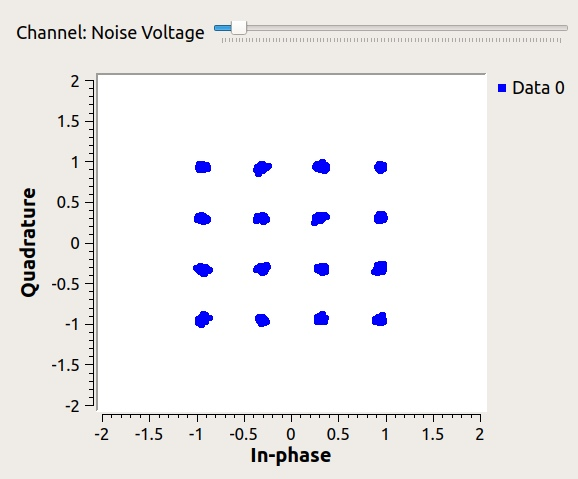
\includegraphics[scale=0.4]{../16qam.jpg}
			\caption{Сигнальное созвездие 16QAM} 
		\end{center}
	\end{figure}
	Как можно видеть, график созвездия подтверждает сказанное выше. Некоторые точки совпадают по фазе, однако, имея различную амплитуду, являются разными дискретными значениями. 
	
	\newpage
	\section{Выводы}
	В ходе выполнения работы были исследованы различные виды цифровых манипуляций. Были выяснены отличия разных видов манипуляций, а также сделаны некоторые выводы:
	\begin{itemize}
		\item можно в разы ускорить передачу данных, используя другой вид манипуляции
		\item чем больше передается информации, тем больше сказывается шум
		\item главная сложность - найти баланс между скоростью и надежностью
		\item чтобы сделать манипуляции более эффективными, нужно пробовать добавлять помехоустойчивое кодирование
		\item фазовый сдвиг может влиять на качество передачи, однако зависит от характеристик канала
	\end{itemize}
	Таким образом, работа над цифровыми манипуляциями "приоткрывает завесу тайны" над теми устройствами и технологиями, которыми мы пользуемся каждый день. Именно с помощью нахождения баланса между кодированием, манипуляциями и другими параметрами каналов и оборудования сейчас доступны беспроводные высокоскоростные сети. Каждая подобная технология является не только набором различных методов и устройств, но и их динамической комбинацией, как, например, смена цифровой манипуляции "на лету" в Wi-Fi для обеспечения нормальной передачи информации. Все эти достижения и развитие в целом обусловлены, зачастую, очень интересными и по-своему простыми решениями, в частности, цифровыми манипуляциями.
\end{document}